\onecolumn
\section*{Anaylsis of the Issue}

\begin{figure}[H]
     \centering
     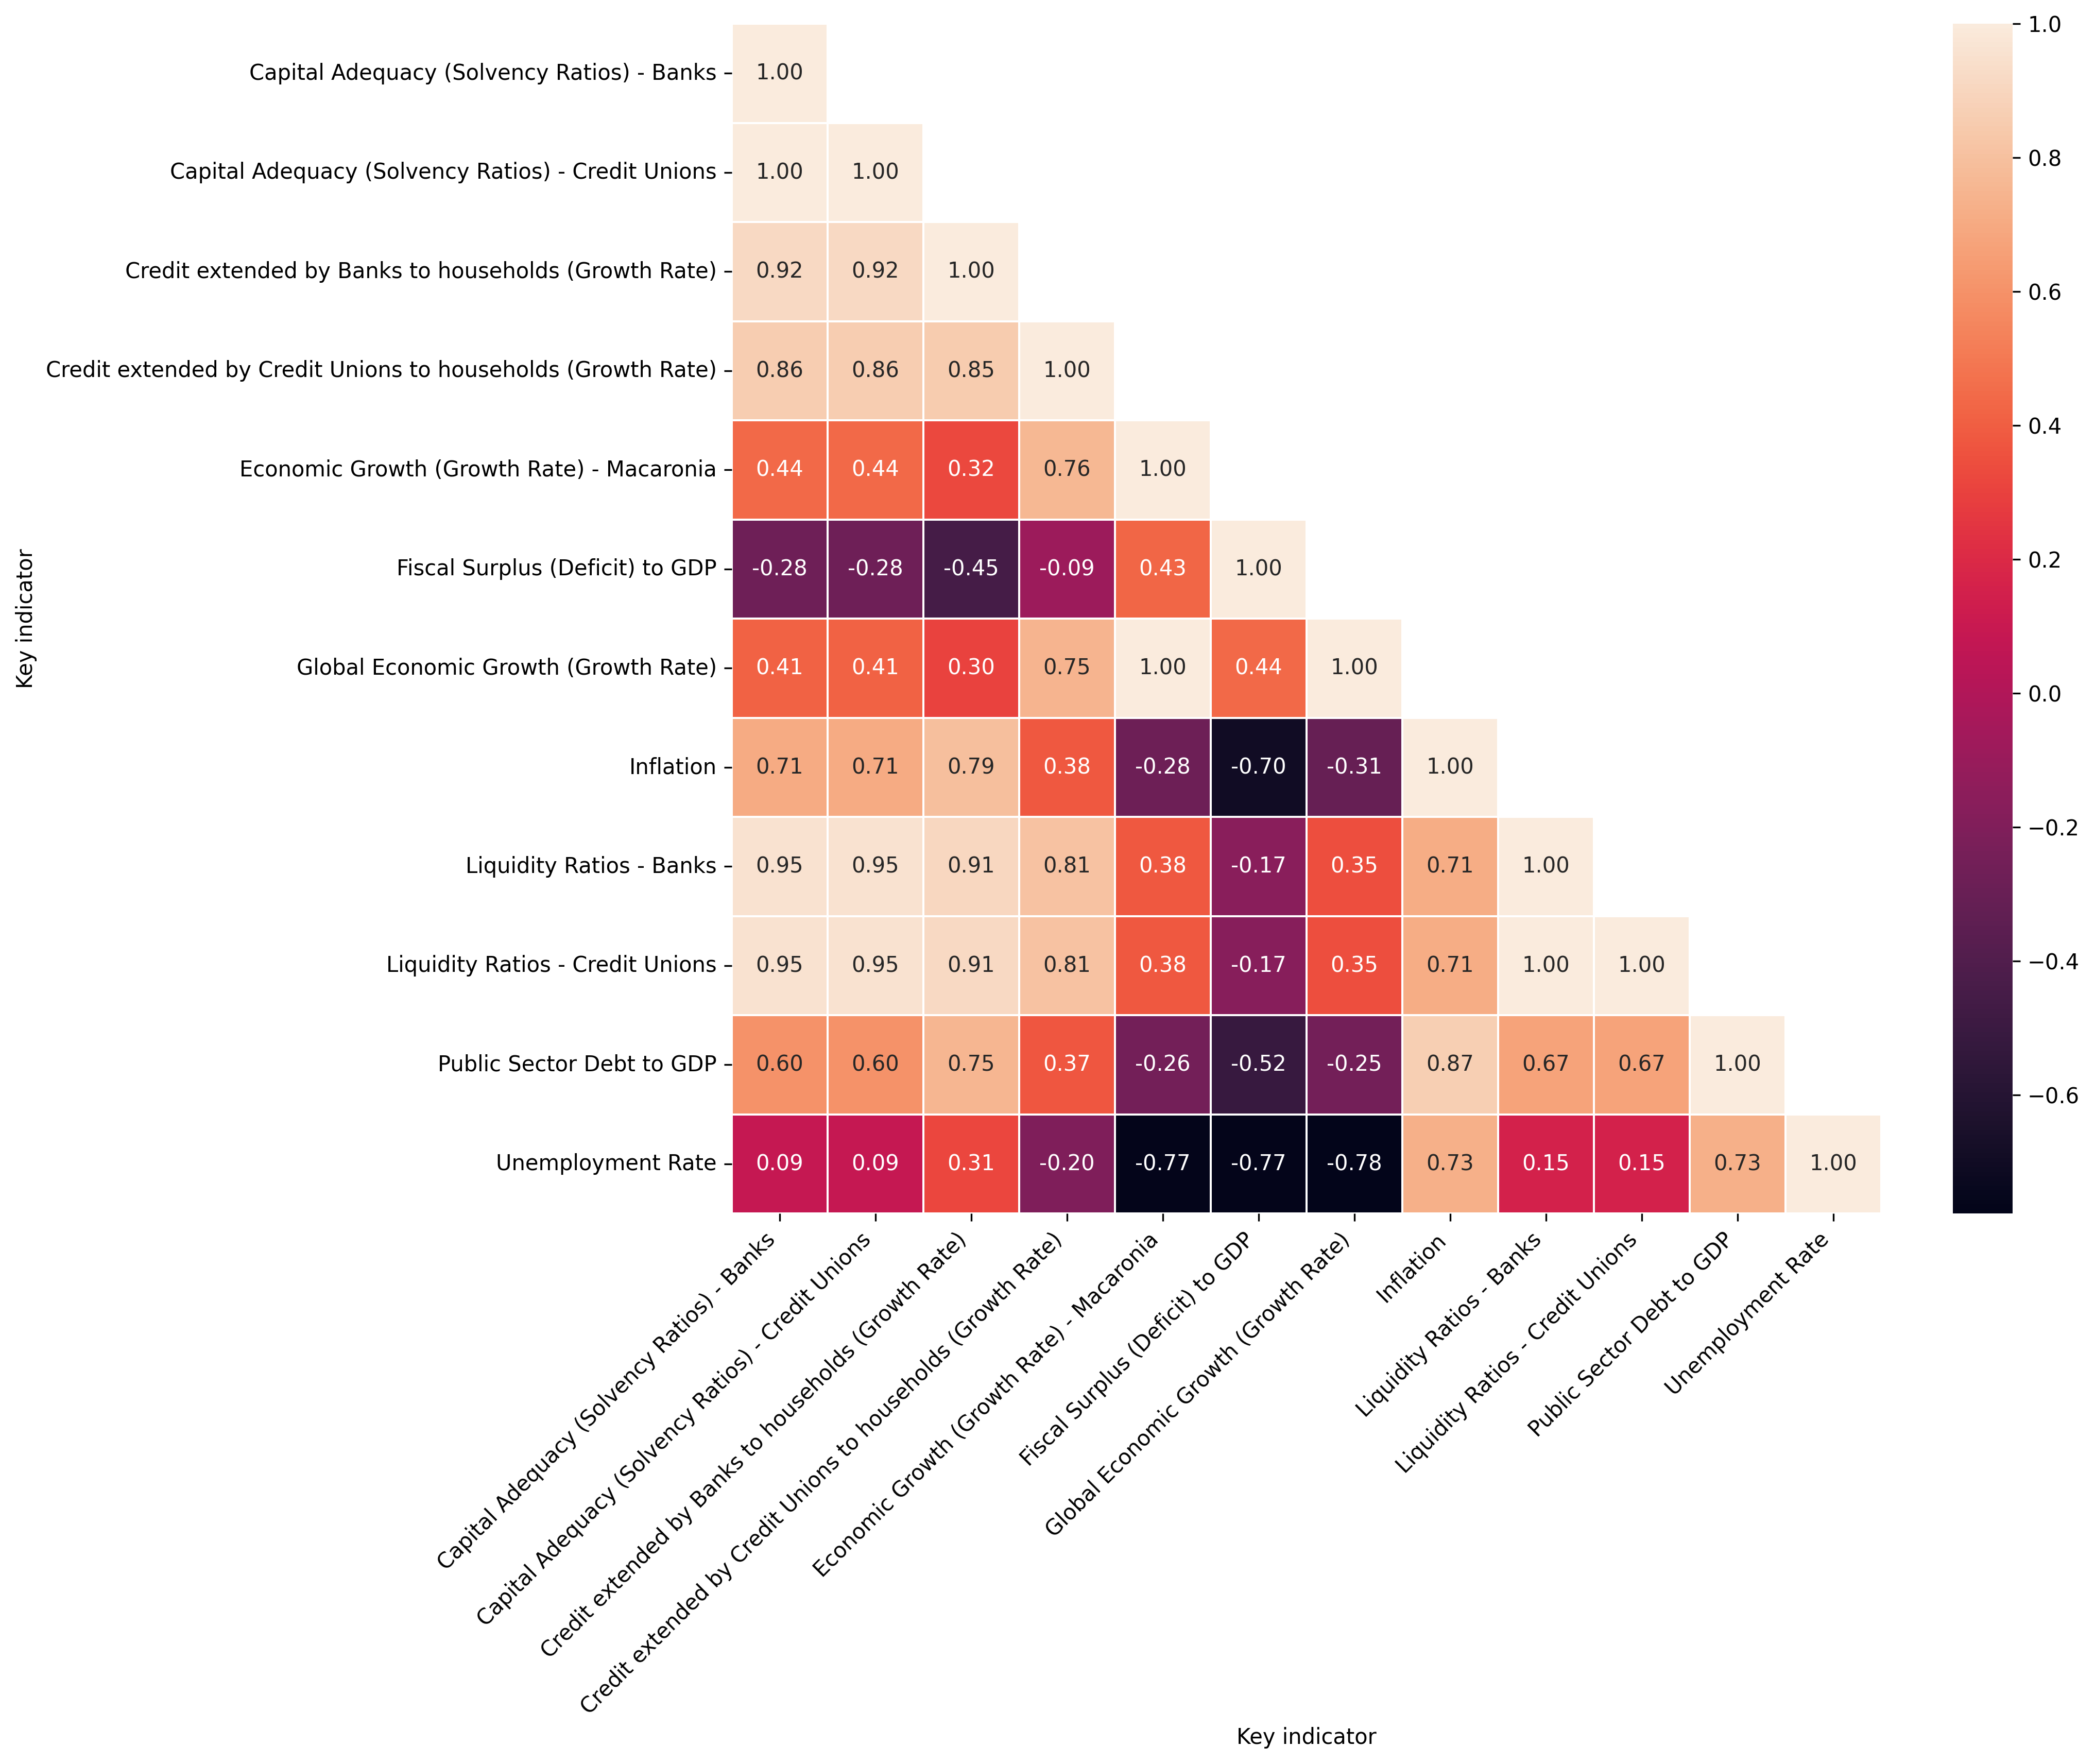
\includegraphics[width=0.86\textwidth]{correlation_matrix.png} % Include the image
     \caption{Correlation Matrix Heatmap}
     \label{fig:correlation_matrix}
\end{figure}


Macaronia’s economic crisis was driven by an aggressive push for growth, but the foundations supporting that growth were far from stable. 
This section begins by assessing the true financial health of banks and credit unions, adjusting their liquidity and capital adequacy ratios to account for credit expansion and risk exposure.
It then examines how heavy investments in REITs heightened financial vulnerabilities, making institutions more susceptible to market shocks. Finally, it explores the key events that triggered the crisis, 
the role of external financial pressures, and the lasting consequences on Macaronia’s economy.


